\documentclass[book]{jlreq}

\usepackage{graphicx}
\usepackage{amsmath,amssymb,amsthm}
%\usepackage{mathtools}
%%\usepackage{siunitx}
\usepackage{physics}
\usepackage{bm}

\renewcommand{\today}{\the\year/\the\month/\the\day}
\renewcommand{\contentsname}{Contents}
\renewcommand{\refname}{References}
\renewcommand{\figurename}{Fig.~}
\renewcommand{\tablename}{Table~}

\begin{document}
\title{Beam Loading}
\author{Shin-ichi YOSHIMOTO}
\maketitle
\tableofcontents
%%\clearpage

\part{Beam Loading}
\chapter{Static Beam Loading}
\section{Cavityの基礎}
\subsection{Power dissipation}
\begin{equation}
    P_{diss} = \frac{1}{2} \cdot \frac{V_{cav}^2}{R} = \frac{V_{cav}^2}{R_{sh}} 
\end{equation}

\subsection{Shut impedance}
\begin{equation}
    R = \frac{1}{2}\cdot R_{sh}
\end{equation}

空洞の入力カップラーの変圧比を$1:n$とすると(Fig. \ref{fig:Ideal_Trans})、
%
\begin{figure}[hbt]
    \begin{center}
        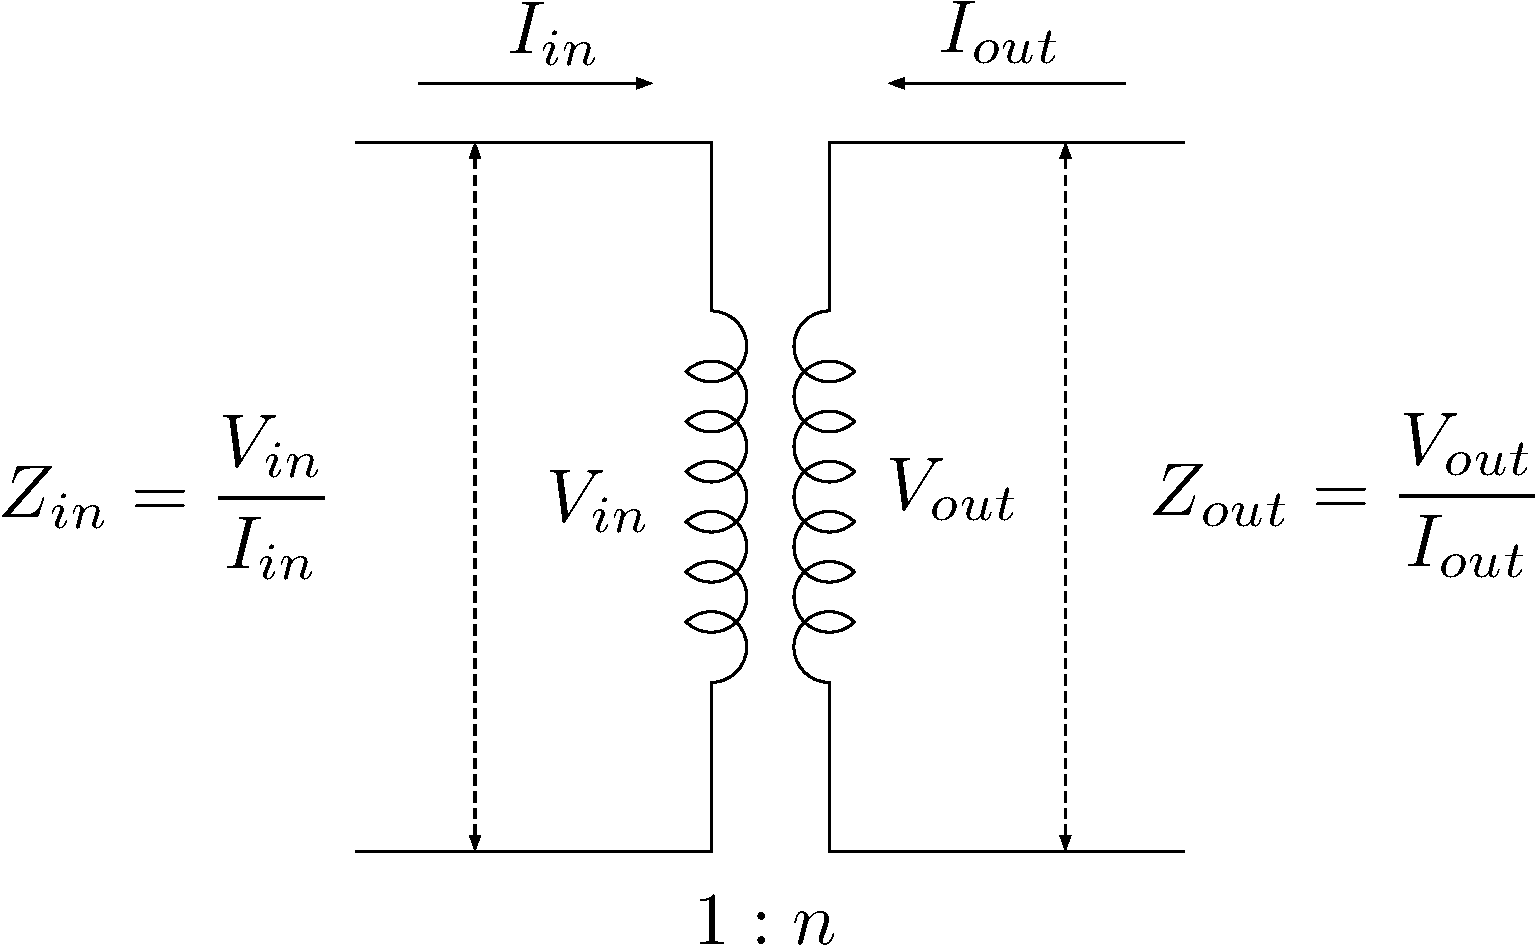
\includegraphics[width=12cm,clip]{figs/Ideal_Transformer.pdf}
        \caption{理想的なトランスによる入力カップラー.}
        \label{fig:Ideal_Trans}
    \end{center}
\end{figure}
%
\begin{equation}
    V_2 = N\cdot V_1, \; I_2 = \frac{1}{N}\cdot I_1
\end{equation}
%
したがって、
\begin{equation}
    Z_2 = n^2 \cdot Z_1 
\end{equation}


\section{ビーム負荷付き空洞のRCL等価回路}

\begin{figure}[hbt]
    \begin{center}
      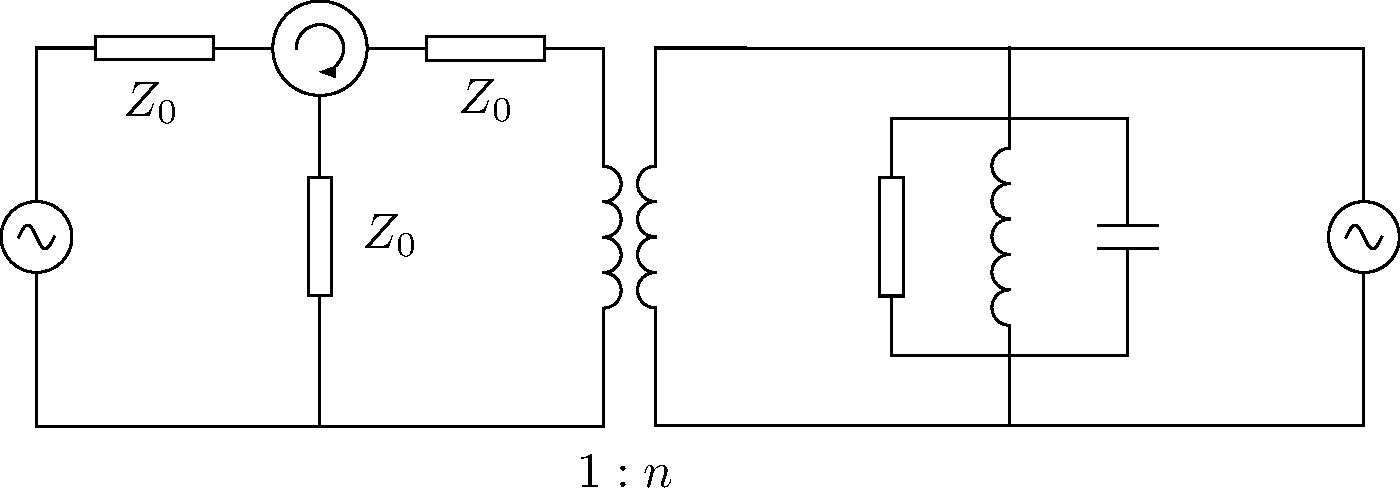
\includegraphics[width=12cm,clip]{figs/Cavity_Model.pdf}
      \caption{理想的なトランスによる入力カップラー.}
     \label{Cavity_Model}
    \end{center}
\end{figure}

\subsection{Cavity parameters}

\begin{figure}[hbt]
    \begin{center}
      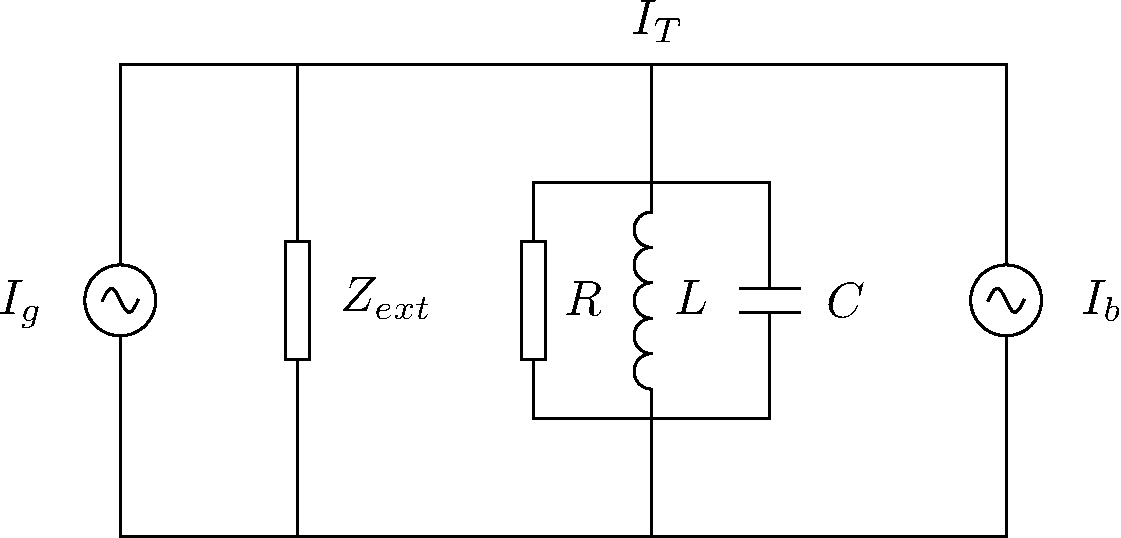
\includegraphics[width=12cm,clip]{figs/Equivalent_Circuit}
      \caption{等価回路}
     \label{Equivalent_Circuit}
    \end{center}
\end{figure}
%
\paragraph{共振周波数}
%
\begin{equation}
    \omega_0 = \frac{1}{L C}
\end{equation}
%
\paragraph{Quality factor}
%
\begin{equation}
    Q = 2\pi \frac{\mathrm{stored\;energy\;in\;cavity}}{\mathrm{dissipated \; energy\;per\;cycle}} = \frac{\omega_0 W}{P_{diss}}
\end{equation}
%
\paragraph{Unloaded quality factor}
%
\begin{equation}
    Q_0 = \omega_0 \frac{(1/2) C V^2}{V^2/(2R)} = \omega_0 R C 
\end{equation}
%
\paragraph{External quality factor}
%
\begin{equation}
    Q_{ext} = 2\pi \frac{\mathrm{stored\;energy\;in\;cavity}}{\mathrm{dissipated \; energy\;in\;external\;devices\;per\;cycle}}
     = \frac{\omega_0 W}{P_{ext}}
\end{equation}
%
\paragraph{Loaded quality factor}
%
\begin{equation}
    Q_L = 2\pi \frac{\mathrm{stored\;energy\;in\;cavity}}{\mathrm{total \; energy\;per\;cycle}} = \frac{\omega_0 W}{P_{tot}}
\end{equation}
%
ここで、
%
\begin{equation}
    P_{tot} = P_{diss} + P_{ext}
\end{equation}
%
したがって、
%
\begin{equation}
    \frac{1}{Q_L} = \frac{1}{Q_0} + \frac{1}{Q_{ext}}
\end{equation}
%
\begin{equation}
    \frac{1}{R_L} = \frac{1}{R} + \frac{1}{Z_{ext}}
\end{equation}
%
\paragraph{Coupling factor \beta}
%
\begin{equation}
    \beta = \frac{P_{ext}}{P_{cav}} = \frac{Q_0}{Q_{ext}} = \frac{R}{Z_{ext}} = \frac{R}{n^2 Z_0}
\end{equation}
%
\begin{figure}[hbt]
    \begin{center}
      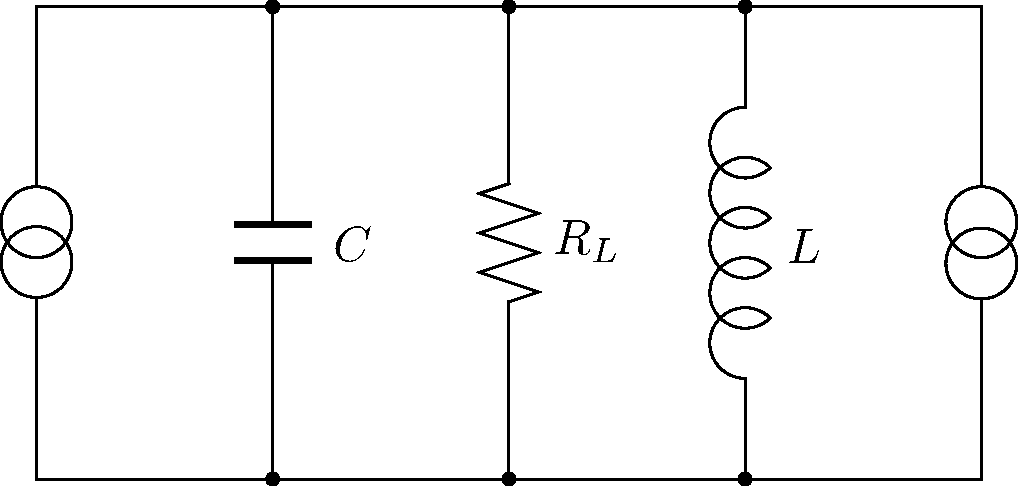
\includegraphics[width=12cm,clip]{figs/Equivalent_Circuit2}
      \caption{等価回路2}
     \label{Equivalent_Circuit2}
    \end{center}
\end{figure}
%
\begin{equation}
    \ddot{V}(t) + \frac{1}{R_L C}\dot{V}(t) + \frac{1}{L C} V(t) = \frac{1}{C} \dot{I}(t)
\end{equation}
%
\paragraph{Phasor}
\begin{equation}
    V(t) = \tilde{V}e^{j\omega_c t}, \; I(t) = \tilde{I}e^{j\omega_c t}
\end{equation}

\section{Pedersen Model \cite{Pedersen} \cite{Ninomiya}}

\begin{figure}[hbt]
    \begin{center}
        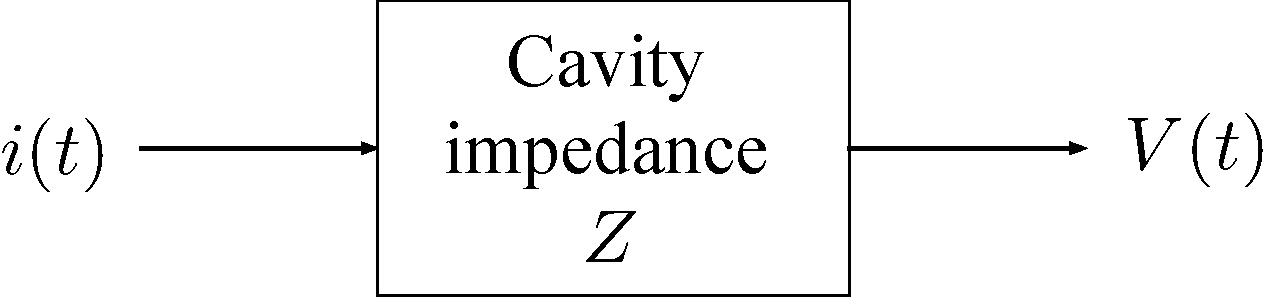
\includegraphics[width=12cm,clip]{figs/Cavity_TF.pdf}
        \caption{加速空洞の伝達関数}
        \label{fig:Cavity_TF}
    \end{center}
\end{figure}

振幅が$a(t)$、位相が$p(t)$で変調された信号$i(t)$は、次のようにあらわせる\cite{Pedersen}。
%
\begin{equation}
    i(t) = \Re{\hat{I}(1 + a_i(t))e^{j(\omega_c t + p_i (t))}}
    \label{eq:input_sig}
\end{equation}
%
伝達関数(インピーダンス)$Z(s)$を通じて出力される信号も一般的に振幅と位相が変調され次のようになれる。
%
\begin{equation}
    V(t) = \Re{\hat{V}(1 + a_v(t))e^{j(\omega_c t + \phi_z + p_v (t))}}
    \label{eq:output_sig}
\end{equation}
%
$a_i(t) \ll 1,\; p_i(t) \ll 1$の時、$e^{j p_i (t)} \simeq 1+j p_i(t)$、および、二次の微少量を無視すると、
%
\begin{align}
    i(t) &=\Re{\hat{I}(1 + a_i(t))(1 + j p_i (t))e^{j\omega_c t}} \notag \\ 
        &=\Re{\hat{I}(1 + a_i(t)+ j p_i (t))e^{j\omega_c t}} \notag \\ 
        &= \hat{I}\{\cos\omega_c t + a_i(t)\cos\omega_c t - p_i(t)\sin\omega_c t\} \notag \\
        &= \frac{\hat{I}}{2}\left \{(e^{j\omega_c t}+e^{-j\omega_c t})+a_i(t)(e^{j\omega_c t} 
        + e^{-j\omega_c t})+ j p_i(t)(e^{j\omega_c t}-e^{-j\omega_c t})\right \}
        \label{eq:input_sig2}
\end{align}
%
$I(s)=\mathcal{L}\{i(t)\},\; a_i(s) = \mathcal{L}\{a_i(t)\},\; p_i(s) = \mathcal{L}\{p_i(t)\}$とし、(\ref{eq:input_sig})をラプラス変換すると、
%
\begin{equation}
    \begin{split}
        I(s) &= \frac{\hat{I}}{2}\biggl [\frac{1}{s-j\omega_c}+\frac{1}{s+j\omega_c} \\
        &+ a_i(s - j\omega_c)+a_i(s+j\omega_c) 
        + j\left \{p_i(s-j\omega_c)-p_i(s+j\omega_c) \right \} \biggr ]
    \label{eq:lt_input}
    \end{split}
\end{equation}
%
同様にして、(\ref{eq:output_sig})をラプラス変換すると、
%
\begin{equation}
    \begin{split}
        V(s) &= \frac{\hat{V}}{2}\biggr [\frac{e^{j\phi_z}}{s-j\omega_c}+\frac{e^{-j\phi_z}}{s+j\omega_c} \\
        &+ e^{j\phi_z}a_v(s - j\omega_c) + e^{-j\phi_z}a_v(s+j\omega_c)
        + j\left \{e^{j\phi_z}p_v(s-j\omega_c) - e^{-j\phi_z}p_v(s+j\omega_c) \right \} \biggl ]
    \label{eq:lt_output}
    \end{split}
\end{equation}
%
ここで、振幅と位相の変調の伝達関数$G(s)$を以下のように定義すると、

変調の伝達は、システムの伝達関数$Z(s)$から導き出すことができる。4つの変調伝達関数のセットを計算する必要があります。

システム解析には、このような変調が増幅器と空洞共振器を介して伝達されることを知ることが必要です。完全な特性評価には4つの異なる伝達関数が必要です。

低変調指数($a \ll 1, p \ll 1$)の場合、変調のトランスミッションは線形であり、次式で決定される。
%
\begin{enumerate}
    \item $G_{aa}(s)$ : 
    \item $G_{pp}(s)$ :
    \item $G_{ap}(s)$ :
    \item $G_{pa}(s)$ :
\end{enumerate}
%
\begin{equation}
    \left\{
    \begin{matrix}
        a_y(s) = G_{aa}(s) a_x(s) + G_{pa}(s) p_x(s)\\
        p_y(s) = G_{ap}(s) a_x(s) + G_{pp}(s) p_x(s)
        \label{eq:amfm_tf}
    \end{matrix}
    \right .
\end{equation}
%
(\ref{eq:amfm_tf})を(\ref{eq:lt_output})に代入すると
%
\begin{equation}
    \begin{split}
        V(s) &= \frac{\hat{V}}{2}\biggl [ \frac{e^{j\phi_z}}{s-j\omega_c}+\frac{e^{-j\phi_z}}{s+j\omega_c} \\
        &+ e^{j\phi_z}\bigl \{G_{aa}(s-j\omega_c)a_i(s-j\omega_c) + G_{pa}(s-j\omega_c) p_i(s-j\omega_c) \bigr \} \\
        &+ e^{-j\phi_z}\bigl \{G_{aa}(s+j\omega_c)a_i(s+j\omega_c) + G_{pa}(s+j\omega_c) p_i(s+j\omega_c) \bigr \} \\
        &+ j e^{j\phi_z}\bigl \{G_{ap}(s-j\omega_c)a_i(s-j\omega_c) + G_{pp}(s-j\omega_c)p_i(s-j\omega_c) \bigr \}\\
        &- j e^{-j\phi_z}\bigl \{G_{ap}(s+j\omega_c)a_i(s+j\omega_c) -G_{pp}(s+j\omega_c)p_i(s+j\omega_c)\bigr \} \biggr ] \\
        &= \frac{\hat{V}}{2}\biggl [ \frac{e^{j\phi_z}}{s-j\omega_c}+\frac{e^{-j\phi_z}}{s+j\omega_c} \\
        &+ e^{j\phi_z}\{G_{aa}(s-j\omega_c)+j G_{ap}(s-j\omega_c)\}a_i(s-j\omega_c) \\
        &+ e^{-j\phi_z}\{G_{aa}(s+j\omega_c)-j G_{ap}(s+j\omega_c)\}a_i(s+j\omega_c) \\
        &+ e^{j\phi_z}\{G_{pa}(s-j\omega_c) + j G_{pp}(s-j\omega_c)\}p_i(s-j\omega_c) \\
        &+ e^{-j\phi_z}\{G_{pa}(s+j\omega_c) + j G_{pp}(s+j\omega_c)\}p_i(s+j\omega_c)\biggr ]
    \end{split}
    \label{eq:Vc1}
\end{equation}
%
ここで、
%
\begin{equation}
    \begin{split}
        V(s) = Z(s) I(s) &= \frac{Z(s)\hat{I}}{2} \biggl [\frac{1}{s-j\omega_c}+\frac{1}{s+j\omega_c} \\ 
        &+ a_i(s - j\omega_c) + a_i(s+j\omega_c) + j\left \{p_i(s-j\omega_c)-p_i(s+j\omega_c) \right \} \biggr ]
    \end{split}
    \label{eq:Vc2}
\end{equation}
%
(\ref{eq:Vc1})と(\ref{eq:Vc2})で、係数を比較すると、
%
\begin{equation} 
    \hat{V}\left(\frac{e^{j\phi_z}}{s-j\omega_c} + \frac{e^{-j\phi_z}}{s+j\omega_c} \right) =
    Z(s)\hat{I}\left(\frac{1}{s-j\omega_c} + \frac{1}{s+j\omega_c}  \right) \\
    \label{eq:coef1}
\end{equation}
%
\begin{equation}
    \begin{split}
        G_{aa}(s-j\omega_c) + j G_{ap}(s-j\omega_c) &= \frac{\hat{I}}{\hat{V}}e^{-j\phi_z}Z(s) \\
        G_{aa}(s+j\omega_c) - j G_{ap}(s+j\omega_c) &= \frac{\hat{I}}{\hat{V}}e^{j\phi_z}Z(s) \\
        G_{pa}(s-j\omega_c) + j G_{ap}(s-j\omega_c) &= j \frac{\hat{I}}{\hat{V}}e^{-j\phi_z}Z(s) \\
        G_{pa}(s+j\omega_c) - j G_{ap}(s+j\omega_c) &= -j \frac{\hat{I}}{\hat{V}}e^{j\phi_z}Z(s) 
    \end{split}
\end{equation}
%
(\ref{eq:coef1})を整理すると、
%
\begin{equation}
    Z(s) = \frac{2 s \hat{V}}{\hat{I}}\left\{e^{j\phi_z}(s+j\omega_c)+e^{-j\phi_z}(s-j\omega_c)\right\}
\end{equation}
%
したがって、
%
\begin{equation}
    \begin{split}
        G_{aa}(s) + j G_{ap}(s) &= \frac{Z(s+j\omega_c)}{Z(j\omega_c)} \\
        G_{aa}(s) - j G_{ap}(s) &= \frac{Z(s-j\omega_c)}{Z(-j\omega_c)} \\
        G_{pa}(s) + j G_{ap}(s) &= j \frac{Z(s+j\omega_c)}{Z(j\omega_c)} \\
        G_{pa}(s) - j G_{ap}(s) &= -j \frac{Z(s-j\omega_c)}{Z(-j\omega_c)} 
    \end{split}
\end{equation}
%
これらより、
%
\begin{equation}
    \begin{split}
        G_{aa}(s) &= G_{pp}(s)  = \frac{1}{2}\left\{\frac{Z(s+j\omega_c)}{Z(j\omega_c)} + \frac{Z(s-j\omega_c)}{Z(-j\omega_c)}\right\} \\
        G_{pa}(s) &= - G_{ap}(s) = \frac{j}{2}\left\{\frac{Z(s+j\omega_c)}{Z(j\omega_c)} - \frac{Z(s-j\omega_c)}{Z(-j\omega_c)}\right\}
    \end{split}
\end{equation}
%
\begin{thebibliography}{9}
    \bibitem{Pedersen}
    F. Pedersen, Beam Loading Effects in the CERN PS Booster, IEEE Trans. Nucl. Sci. 22, 3, June 1975.
    \bibitem{Ninomiya}
    S. Ninomiya, Beam Loading Effect on RF System in Proton Synchrotrons, KEK Report 89-18 (1989).
    \bibitem{llrf}
    S. Simrock, Z. Geng, Low-Level Radio Frequency Systems, Springer (2022)
    \bibitem{Schilcher}
    T. Schilcher Vector sum control of pulsed accelerating fields in Lorentz force detuned superconducting cavities (1998).
    \bibitem{Wilson}
    P. B. Wilson, High energy electron linacs; application to storage ring RF systems and linear colliders (1987)
\end{thebibliography}
%
%
\end{document}